\section{Results}
\label{sec:results}

The first thing we measured was the convergence rate of Jacobi's algorithm, see Figure \ref{fig:n_vs_it}.
We see that after some fluctuations for low n, the curve becomes as n increases.
As this is in logspace, we have that the convergence rate slows down exponentially
for higher n.
\begin{figure}[htbp]
	\centering
	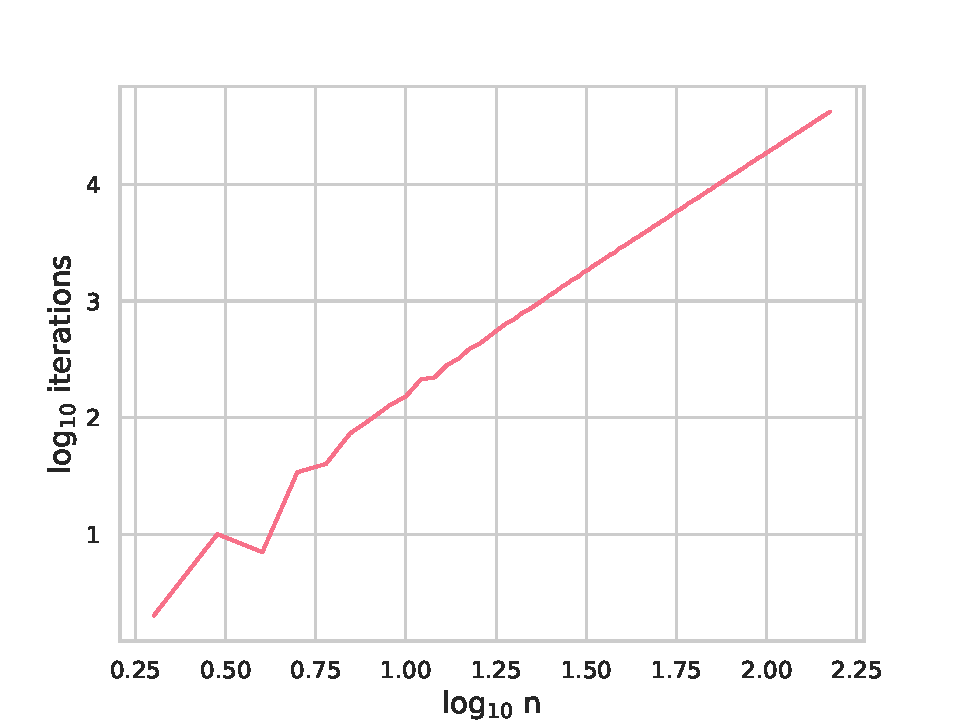
\includegraphics[width=0.5\textwidth]{n_vs_itterations.pdf}
	\caption{Number of iterations used for solving the buckling beam as a function of the matrix dimension n with a logarithmic scale. The slope of the linear fit is 2.11.}
	\label{fig:n_vs_it}
\end{figure}

In Figure \ref{fig:CPUtime} we compare the CPU time between Jacobi's method and
armadillo's built-in eigenvalue solver, where we see that the CPU time of Jacobi's method
has a similar shape as in Figure \ref{fig:n_vs_it}. Looking at the graph for the armadillo
function we see that the slope is less steep
\begin{figure}[htbp]
	\centering
	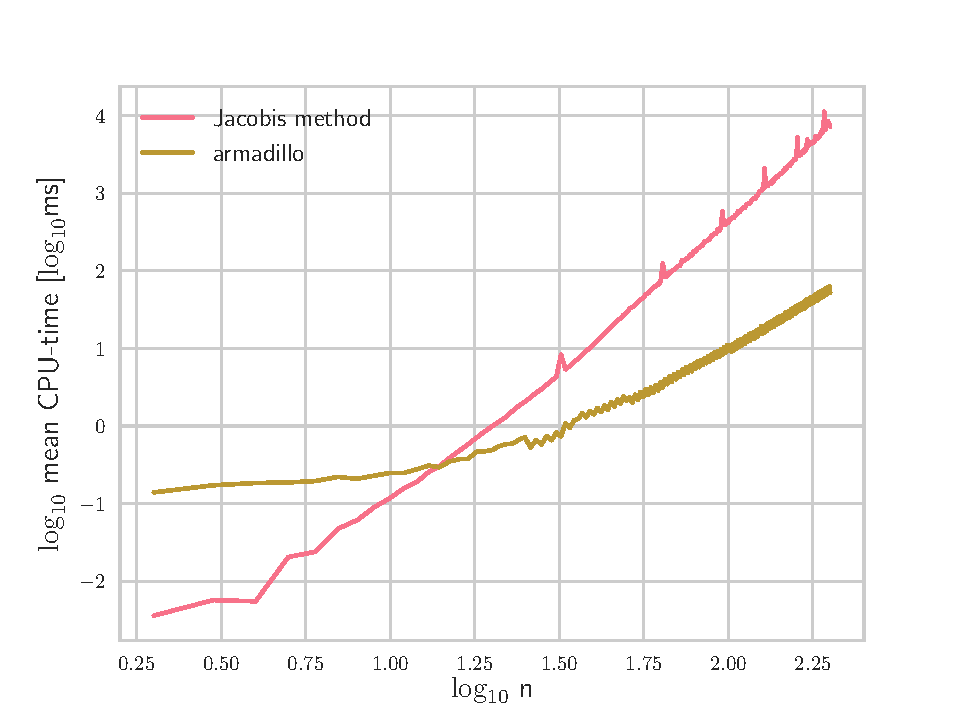
\includegraphics[width=0.5\textwidth]{CPU_time.pdf}
	\caption{CPU time in ms for solving the buckling beam as a function the matrix dimension n. Both Jacobi's method (red) and armadillo's \texttt{eig\_sym} function (yellow-green) is shown. The scale is logarithmic.}
	\label{fig:CPUtime}
\end{figure}

\begin{figure}[htbp]
	\centering
	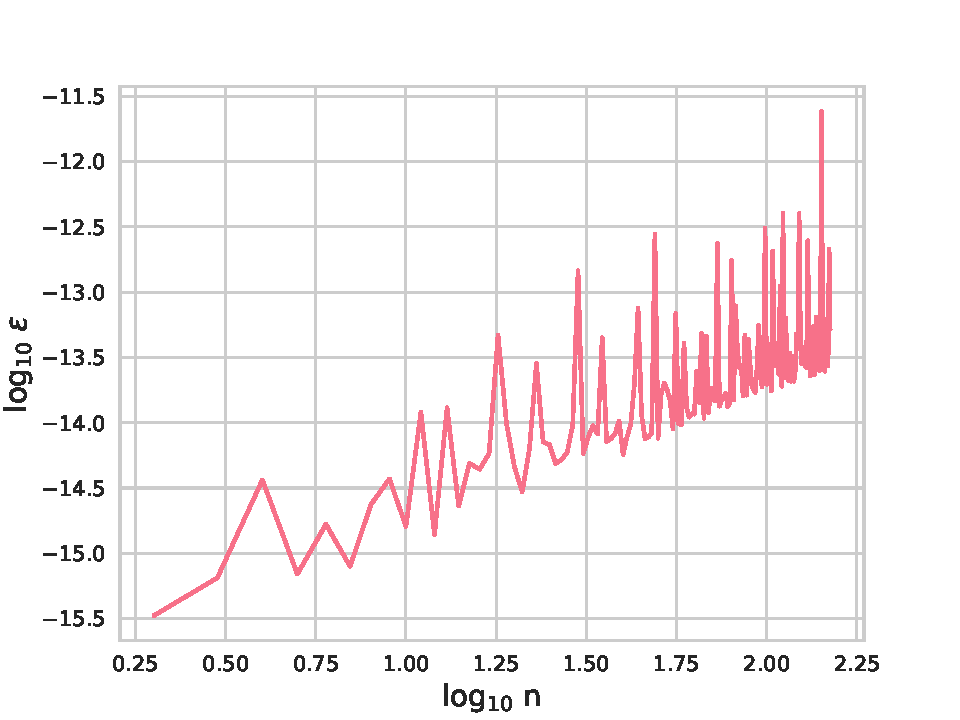
\includegraphics[width=0.5\textwidth]{relative_error.pdf}
	\caption{Maximum relative error, $\epsilon_{max}$ of Jacobi's algorithm applied on the buckling beam problem.
	Here $n$ is the matrix dimension, and the scale is logarithmic.}
	\label{fig:error}
\end{figure}
